\section{Implementation}\label{sec:implementation}
\subsection{Parking garage}\label{sec:implementation-parking-garage}
For the demonstration a working model of the \ac{ips} has to be made. Since it isn't in the scope of the project to create a full scale working parking garage a scaled down model of a parking garage was created to show the functionalities of the \ac{ips}. The scale model has to meet the following set of requirements: it has to have a sufficient amount of parking spaces to show the functionalities as described in subsection \ref{sec:core-functionalities}. It has to have working barriers to let cars enter and exit the parking garage, it has to have indication lights to show if a parking spot is occupied/reserved or available.

\subsubsection{Scale model}
The model has six parking lots that each have a cutout for the \acp{udms}, which will detect if a car is occupying a parking lot as well as cutouts for the indication lights that will be green if the parking space is available and red if it is either occupied or reserved. There is a small entrance/exit road equipped with two barriers controlled by servo motors to stop cars from entering if there are no available spaces left in the parking garage, or to stop cars from exiting if they have not payed yet. Above the barrier is a horizontal beam that will be used to mount the camera for taking images of the licence plates of the entering and exiting cars. On the entrance side of the entrance/exit road is a \ac{lcd} display that shows the number of available spaces in the garage. Underneath the parking spaces is an empty space that can be used to run the wiring and house the raspberry pi.

The scale model was laser cut out of \ac{mdf}-plates. All parts are secured together using press fit connections so no glue is required. This has the advantage that the different parts can be easily taken apart and modified if needed during the development of the parking system. Figure \ref{fig:parking-garage} shows this scale model of the parking garage.

\begin{figure}[H]
    \centering
    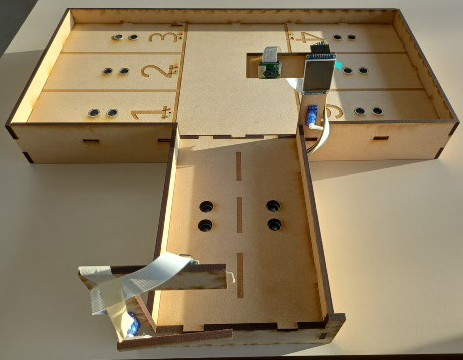
\includegraphics[width=10cm]{images/parking_garage.jpg}
    \caption{Scale model of parking garage}
    \label{fig:parking-garage}
\end{figure}



\subsection{Local garage system}\label{sec:implementation-on-site-system}
There are four main functionalities that the local system should fulfil: 1) identifying cars by their licence plate, 2) detecting cars on parking spots and controlling the signalling \acp{led}, 3) operating the servo motors of the barriers and 4) controlling the \ac{lcd}-display. The backend server acts as a synchronisation for the multiple \ac{iot}-devices in the local garage system, as well as a single source of truth. In the current implementation, the local garages system uses two Raspberry Pi's. Figure \ref{fig:deployment-garage-setup} shows the deployment diagram, with the different modules which run on the Raspberry Pi's.\footnote{In this and the following paragraphs `Raspberry Pi' can be replaced by a more general \ac{iot}-device. The core principles remain the same.}

\subsubsection{Raspberry Pi}
The heart of the local system are two Raspberry Pi's model B\. They runs a 64-bit \ac{os}\footnote{The amount of bits of an operation system is a characteristic of the processor and determines how many memory addresses the \ac{cpu} can access. \ac{cpu}s with 32-bit can access at most $2^{32}$ bytes ($= 4 \ \text{GB}$) of \ac{ram} \cite{bit-cpu}.}. This allows the usage of 64-bit Python packages, like \texttt{torch}\footnote{\url{https://pytorch.org/}}. The four main functionalities are separated into three Python packages\footnote{The code can be found in this GitHub repository: \url{https://github.com/orgs/2022PO3/repositories}.} which run in parallel. This provides a segmented approach to installing all the dependencies of the different packages. Furthermore this makes it possible for the Raspberry Pi to run the multiple services together, making the overall system faster. Figure \ref{fig:general-deployment-diagram} in Appendix \ref{app:deployment-diagram} shows a schematic overview of the interaction between the software on the Raspberry Pi and the hardware components. Figure \ref{fig:deployment-garage-setup} shows the deployment diagram for the garage setup. The first Raspberry Pi will power and control the \ac{lcd}-screen. Besides that, both Raspberry Pi take charge of one half of the parking garage (i.e. one camera, six \acp{led}, four \acp{udms} and one servo motor). The functionalities are subdivided into two main systems (and programs on the Raspberry Pi), namely the \verb|entrance_system|, which handles the entrance and exits of cards and the \verb|parking_lot_system|, which handles the detection of cars. The paragraphs below explain these systems more in depth.

\ind The Raspberry Pi communicates with the backend database with specifically designed \ac{api} endpoints (see Table \ref{tab:url-rpi} in Appendix \ref{app:backend-api-slugs} for more details about the specific \ac{api} endpoints) in order to update the different tables regarding the garages and parking lots. It also needs to be able to query the database, to –- for example –- receive information whether the user has paid or not. 


\begin{figure}[hpt]
    \centering
    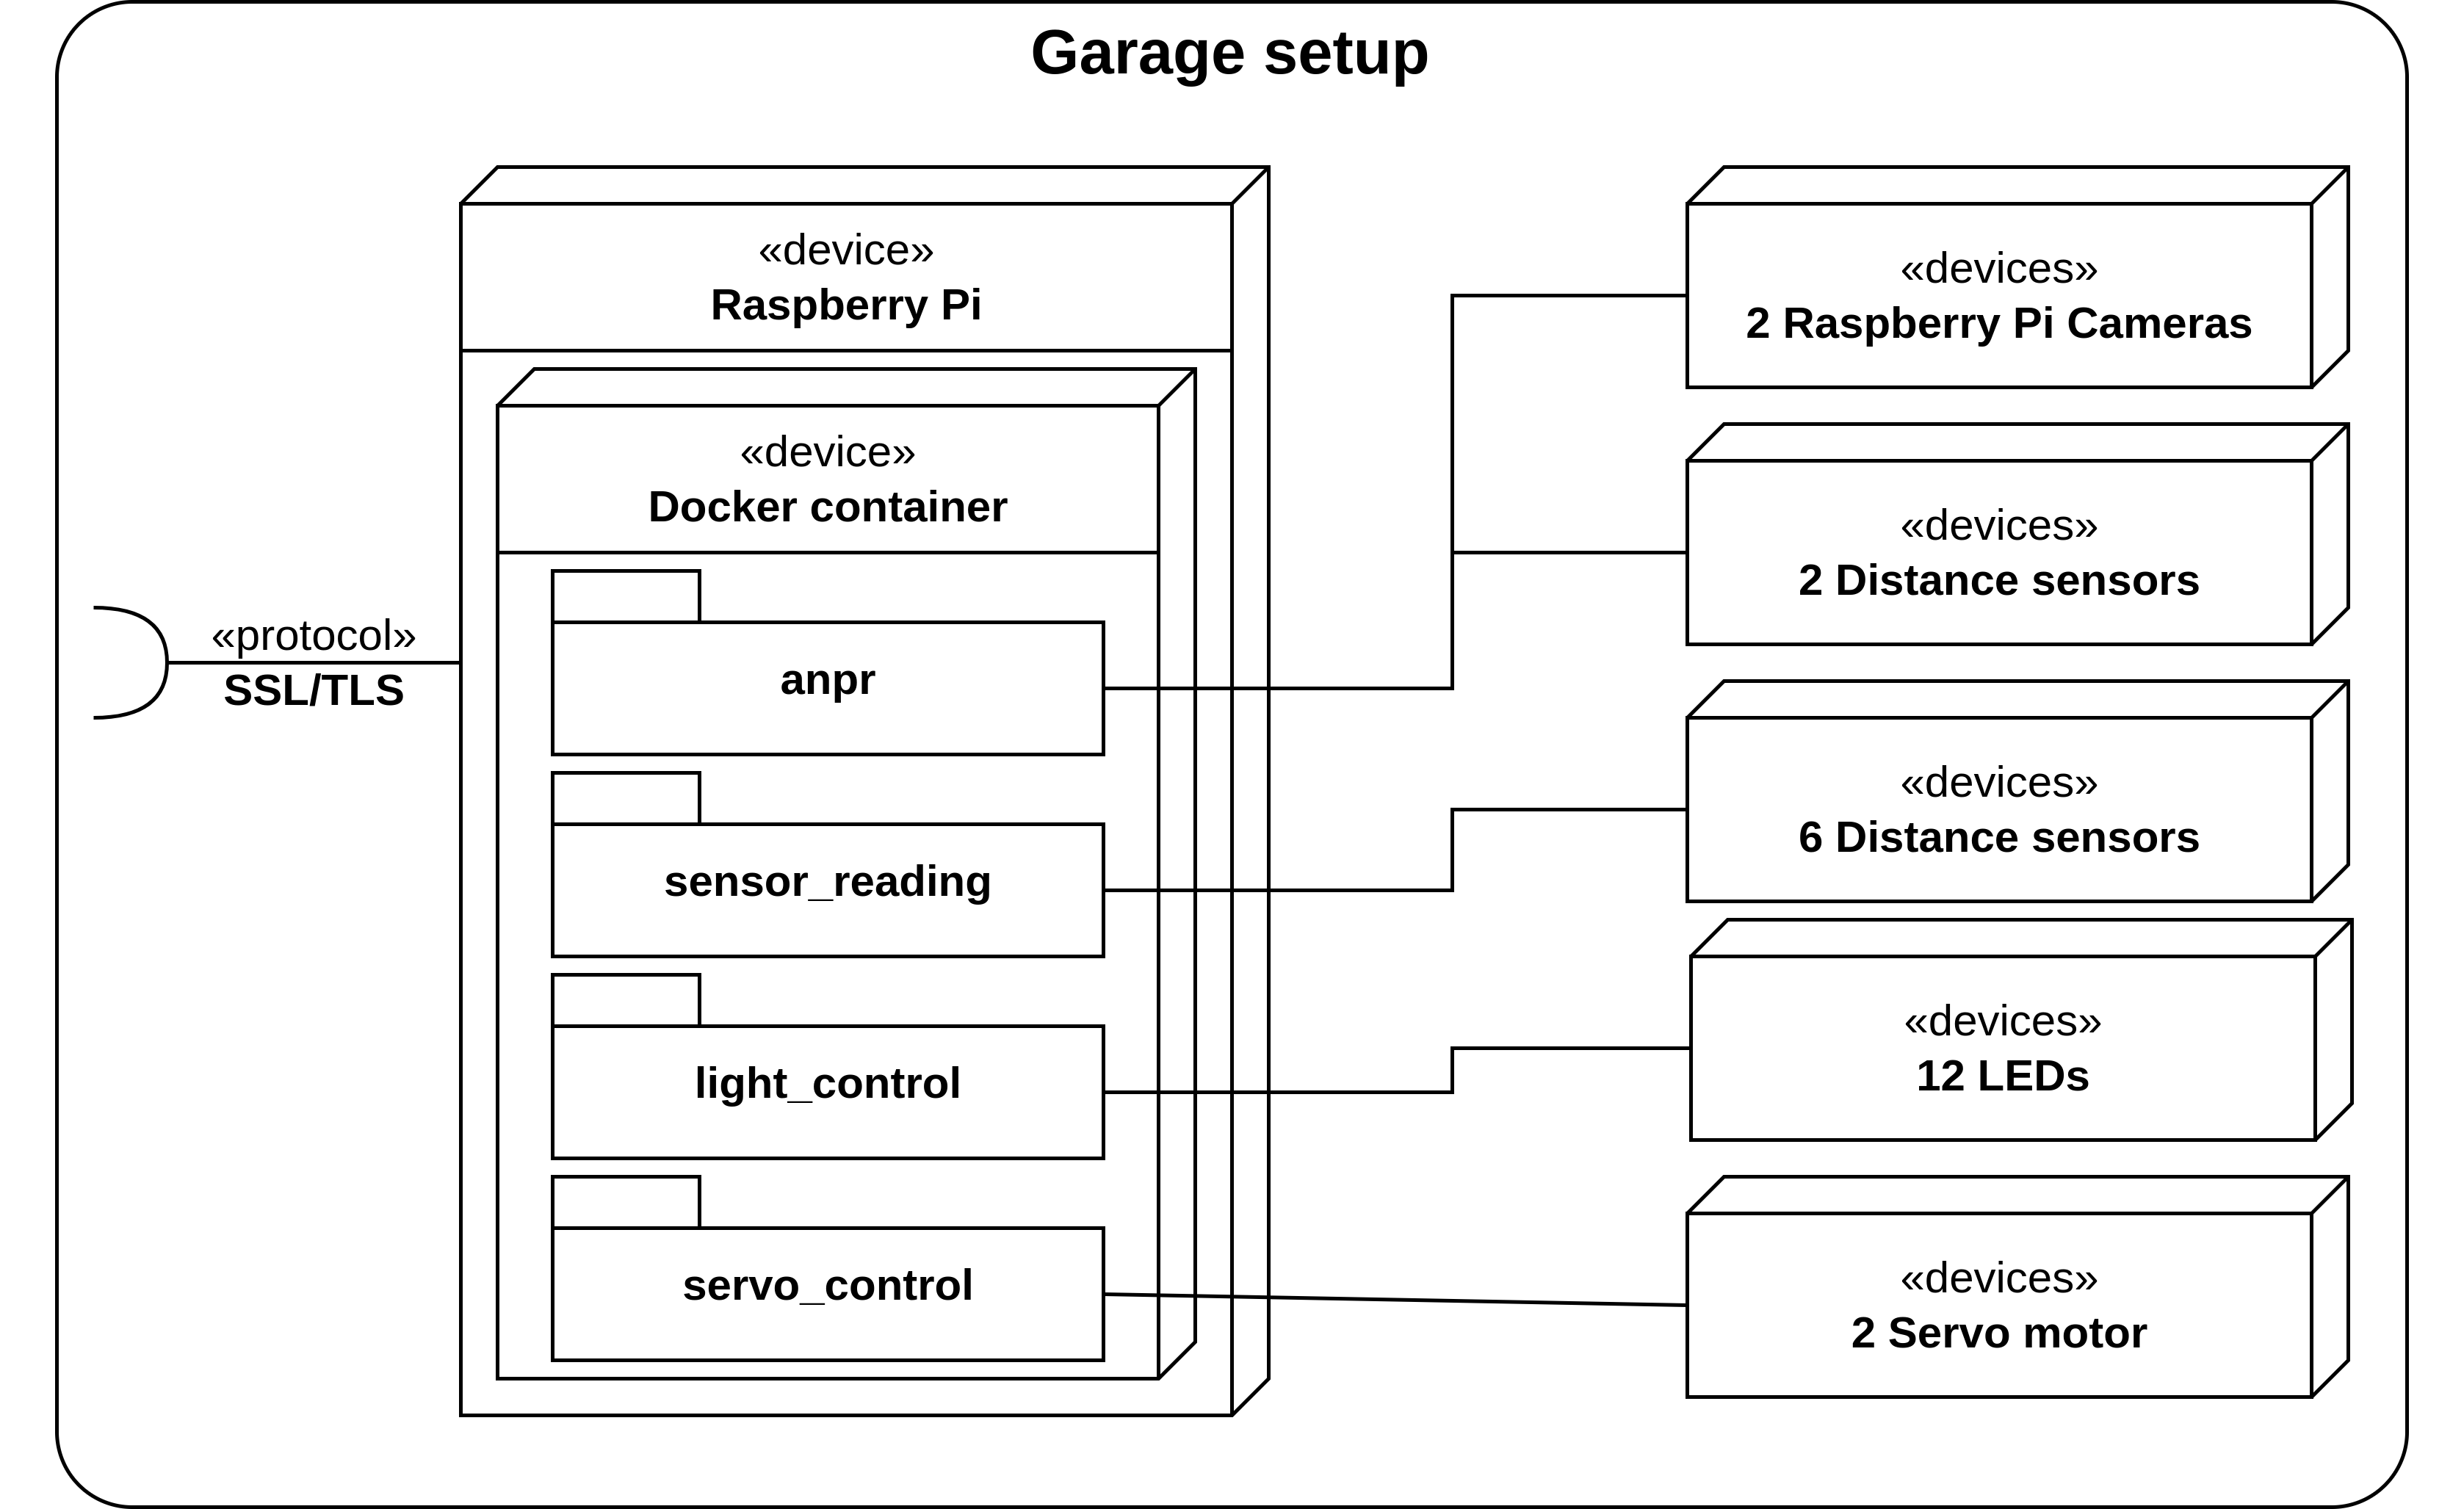
\includegraphics[width=12cm]{images/deployment_diagram_raspberry_pi.png}
    \caption{Deployment diagram of the garage setup.}
    \label{fig:deployment-garage-setup}
\end{figure}

\paragraph{Entrance system}\label{sec:entrance-system}
The local garage system contains two cameras, both powered by a Raspberry Pi. Due to performance issues, the Raspberry Pi will only take a picture of the car and send the picture to the backend, which in turn executes the \ac{anpr} (see Section \ref{sec:anpr} fore more details). 

\ind The taking of the image is triggered by an \ac{udms}. The \verb|udms_control| remembers the previous state of the \ac{udms}. If the current state differs from the current state, a picture is taken with a Bash script, the enhance speed. The image itself is sent to the backend. If the Raspberry Pi receive a positive status code (i.e \verb|200 OK|), \verb|servo_control| will open the barrier and close it after the car has past. Automatically, the amount of free spots will drop by one in the backend due the successful posting of the licence plate image.

\ind The same procedure applies to the exit camera, but here the backend provides an additional check to confirm that the licence plate has paid. If not, the barrier will not open and the user will be notified in the frontend application that the payment has to be fulfilled before he/she can exit the garage. Automatically, the amount of free spots will increase by one in the backend due the successful posting of the licence plate image.

\ind From the moment that the parking garage is completely full, either by physical cars or by reservations, the entrance system will refuse to enter a new cars, except the ones with a valid reservation.

\ind Figure \ref{fig:sequence-diagram-licence-plate} in Appendix \ref{app:sequence-diagrams} visualises the entrance procedure in detail with a sequence diagram.

\paragraph{Parking lot system}
To know the amount of available parking places and to detect cars at the entrance or exit, the local system needs to be able to sense the presence of a car at a specific location in the garage. This can be done by several sensors. The most useful ones are \ac{udms} or light sensors. The latter is more expensive and does not offer any extra advantages over the \ac{udms}. Therefore the demo garage will use the \ac{udms} (\textsc{hc-sr04}).

\ind The \ac{udms} can measure distance by sending ultrasonic sound waves. After the pulse bounces of an object, it gets detected by the same sensor. Using the time between sending and receiving the pulse, the distance can be calculated because we already know the speed of sound. The reduce the risks of false positives, the Raspberry Pi remembers the last two states of every parking lot. From the moment that it detects a car (i.e. the distance measured is smaller than $5 \ \unit{cm}$) two consecutive times, a request is sent to the backend indicating that the parking lot is occupied and turn the red \ac{led} on. The same procedure happens when a car leaves. 

\ind One Raspberry pi has a second component to the \verb|parking_lot_system|, namely \verb|display_control|, which powers and controls the \ac{lcd}-display. This package will make a request to the backend every 5 seconds for the free parking lots left in the garage and display the amount of free spots left (see Section \ref{sec:system analysis} for a discussion about this method).

\subsection{Frontend}\label{sec:implementation-frontend}
This section describes the implementation of the core functionalities of the frontend as described in Section \ref{sec:core-functionalities}. The frontend application is written in Dart, with the Flutter\footnote{\url{https://flutter.dev/}} framework of Google. Flutter is used, because of its platform independence (it can run both on Android, iOS and web), and its provided type safety and null safety. Further, flutter supports a hot reload feature, which makes it easy to develop an application. The next section gives a rough idea how the app will work when you open it. The application is subdivided in to different pages. Each page is enumerated with a combination of letters and number; a new number indicating a new flow and a new letter indicating a new sub-flow. An overview and a short description of all app pages can be found in Appendix \ref{app:app-diagram}, Table \ref{tab:app-pages}.

\subsubsection{Application design}
The following paragraphs discuss the many functionalities of the frontend application. These functionalities are achieved using a multitude of screens, which are bundled into several flows in the application. Table \ref{tab:app-flows} in Appendix \ref{app:app-diagram} gives an overview of all the major application flows and Figure \ref{fig:general-app-diagram} in Appendix \ref{app:app-diagram} gives a schematic overview of the relations between those screens. Of course, the routes defined in Figure \ref{fig:general-app-diagram} are the ideal routes, given that the user enters valid input, which is not always the case. The frontend application implements rigorous validation, such that all data entered will match the type asked by the backend. If the user enters non-valid information, he/she will not be able to continue and a dialog is displayed to the user container the exact description of the errors. Figure \ref{fig:error-dialogs} in Appendix \ref{app:app-diagram} shows examples of this. Besides signalling errors, pop-ups are also frequently used to display information about the application or about the request the user has made. See Figure \ref{fig:information-dialogs} in Appendix \ref{app:app-diagram} for examples of this.

\ind In general, if a button in the application is pressed which loads in a new screen, a request is sent to the backend to get the information about the user, the garage or the reservation required to construct the page. When information has to be changed in the database, different requests are sent to the backend to post, change or delete information in the database. 

\ind The first page of the application is determined dynamically, based on the authentication state of user. If the user is both authenticated and verified (i.e. the user has logged in \textit{and} has provided a \ac{2fa}-code), they application will open the home page directly and the authentication flow will be skipped. If the use is unauthenticated, the login page is opened and the user has to follow the authentication flow. The third case exists when a user is authenticated, but not yet verified (and has \ac{2fa} enabled for his/her account). In that case, page 0c is opened for the user to submit their \ac{2fa}-code.

\ind The following paragraphs explain the flows in more depth. All referenced figures can be found in Appendix \ref{app:app-diagram}.

\paragraph{Authentication flow}
Depending on if the user if logged in or not, the the login page is the first page the user lands on when opening the application. Here they will have the option to login with either their existing account or to register a new one. If they choose to make a new account, then the register page pops up. On this page users have to fill in their first name, last name, email address and password (a licence plate is later added, see Section \ref{sec:profile-flow}). These credentials are used to create a secure account. The user is required to confirm their password by entering the same password in another text field. This is required for lowering the chances of accidentally typing the wrong password. Once the necessary text fields are submitted, the user will be present in the database, but will not yet be active. An email is then sent to the given email address to verify that is is a real address. This email allows users to activate their account and subsequently log in.

\ind If the account is verified, the user can login by hitting the `Sign in'-button. When authenticated, the homepage will be loaded and the app will make a request to the backend server to load all the possible garages. Whilst the app is connecting with the backend, there will be a progress indicator on the screen and the user will still be able to access other features like the navigation bar.

\paragraph{Home flow}
The home flow describes the options available to the user in the home screen itself. This includes opening the navigation bar, which provides the entry point for all major flows inside the application and checking the notifications (Screenshots 1, 1a and 1b; Figure \ref{fig:home-flow}).

\paragraph{Reservation flow}
The most important flow in the application is the reservation flow. After all the garages have been loaded into the app, the user can select one of the garages to make a reservation. Next the information screen will pop up of the selected garage. On this screen the user can observe the location, the amount spots are left in the garage, the price and the opening hours. If the user is satisfied with this garage, then he/she can book a reservation. There will be the option to choose a licence plate linked to the account (only enabled licence plates are able to make a reservation, see Section \ref{sec:licence-plate-validation}), the time and day of the reservation and an available spot in the garage. The user can choose between selecting a spot and getting a spot assigned at random. In the former, the app requests all available parking lots from the backend, out of which the user can choose one, in the latter, the backend returns a random free parking lot. Hereafter, an overview of the reservation is shown and the user is asked to confirm (Pages 2, 2a, 2b, 2c, 2d; Figure \ref{fig:user-reservation-flow}).

\paragraph{User settings flow}
The user settings flow is reached via the navigation bar in the home screen. The user can add a device in order to execute the \ac{2fa} and credit card details for automatic payment. Also the \ac{2fa} and the automatic payment can be enabled or disabled as soon as a device or payment card is added. (Pages 3, 3a, 3b; Figure \ref{fig:user-settings-flow}).

\paragraph{User reservations flow}
This short flow enables users to view, alter and delete their made reservations. The current active reservation is highlighted in green; past reservations are greyed out. Note that it is possible for user with multiple validated licence plates to have multiple reservations on the same time. Multiple reservations on the same moment with the same licence plate are not allowed. See page 4 on Figure \ref{fig:user-reservation-flow} for more details.

\paragraph{Profile flow}\label{sec:profile-flow}
The user info flow is one of the more elaborate flows. When the user selects the ``Profile" tab in the navigation bar, two options are available: user information and licence plates. On the screen containing the user's info, he/she can change his/her first name, last name, email address and favourite garage name. To change your province or password another screen is shown and in order to delete your account a popup is shown. The favourite garage and the province can optionally be given by the use to enhance their experience as it alters the filtering of garage on the home screen (e.g. garages close to the user's location are displayed first) (Pages 5, 5d, 5d1, 5d2 and 5d3; Figure \ref{fig:profile-flow}).

\ind When the user selects the ``licence plates" button instead of the ``user information", there are several options. A licence plate can be added, which is shown on a popup on page 5a. If this plate already exists in the database and not under the current user's id -- meaning that it is possible someone else registered this licence plate with their account --, there is an option to report this. This to make sure that no one is able to follow the whereabouts of a person based on their licence plate. Furthermore, a licence plate can be enabled, as this is required in order to make a reservation for this vehicle. In order to do this, the vehicle registration document has to be uploaded, which is implemented in the application in order to further improve the user privacy. As this not a regular request to make, page 5b1 adds an explication why it is important to validate the licence plate before it is used (Pages 5a, 5a1, 5a2, 5b, 5b1 and 5c; Figure \ref{fig:profile-flow}).

\paragraph{Garage settings flow}
The garage settings flow is only accessible to users that have the role \verb+GARAGE_OWNER+. These users can see their garages in the navigation bar (Page 1a; Figure \ref{fig:home-flow}). They have the option to either configure their owned garages or they can add a new garage into the database. If the user presses on one of those garages, he/she will be redirected to a new page, where they can configure all the settings of the garage (Pages 6 and 6a; Figure \ref{fig:garage-settings-flow}).

\ind For users who are not familiar using the app or a mobile app in general, there would be a guide in the navigation bar. However, this was not implemented in the final design due to a lack of time. At last there is also an option to sign out of your account. A detailed schematic overview of the entire app can be found in Appendix \ref{app:app-diagram} in Figure \ref{fig:general-app-diagram}. 

\paragraph{Payment flow}

\begin{table}[htp]
    \centering
    \begin{tabular}{|c|p{3cm}|p{10cm}|}
    \hline
         \textbf{Flow no.} & \textbf{Flow name} & \textbf{Short description} \\
         \hline
         \hline
         0 & Authentication flow & Flow for registering, logging in the user and sending the \ac{2fa}-code (Figure \ref{fig:auth-flow}). \\
         \hline
         1 & Home flow & Home page and banner which provides a step-stone for all major flows in the application (Figure \ref{fig:home-flow}).\\
         \hline 
         2 & Reservation flow & For making a reservation by selection a licence plate, a spot and a date and time (Figure \ref{fig:reservation-flow}). \\
         \hline 
         3 & User settings flow & Flow for altering user settings like \ac{2fa} and enabling automatic payments (Figure \ref{fig:user-settings-flow}). \\
         \hline
         4 & User reservations flow & Screen for getting an overview of all user reservations (Figure \ref{fig:user-reservation-flow}). \\ 
         \hline
         5 & Profile flow & Flow for altering user information, e.g. name or password (Figure \ref{fig:profile-flow}). \\
         \hline 
         6 & Garage settings flow & Flow for garage owners which enables altering and adding of garages (Figure \ref{fig:garage-settings-flow}). \\ 
         \hline
         7 & Payment flow & Flow for making payments for a parking (Figure \ref{fig:payment-flow}). \\
         \hline
    \end{tabular}
    \caption{Overview of the major app flows.}
    \label{tab:app-flows}
\end{table}

\subsubsection{Deployment}
The frontend deployment should support two use cases: users who want to download the mobile application and users who want to access the website. \\

Due to Flutter's nature, it can run natively on all major platforms and operating systems. To make the mobile application accessible to the general public, it should be uploaded to the Google Play Store, the Apple App Store and the Microsoft Store. For the purpose of this project, the application will be installed on the devices of the team members. \\

% We should check if this is even possible to do, otherwise, this is total bogus.
The web application should be hosted on a web server, for the users to be able to access the site. The backend already incorporates a web server, namely Nginx\footnote{\url{https://nginx.org/}}. Apart from being a reverse-proxy for the backend, it also hosts the static files (\textsc{html} and \ac{js}). Figure \ref{fig:deployment-frontend} shows the deployment diagram for the frontend application. Note that the two client devices represent both options of the client of connection to our backend \ac{api}.


\begin{figure}[H]
    \centering
    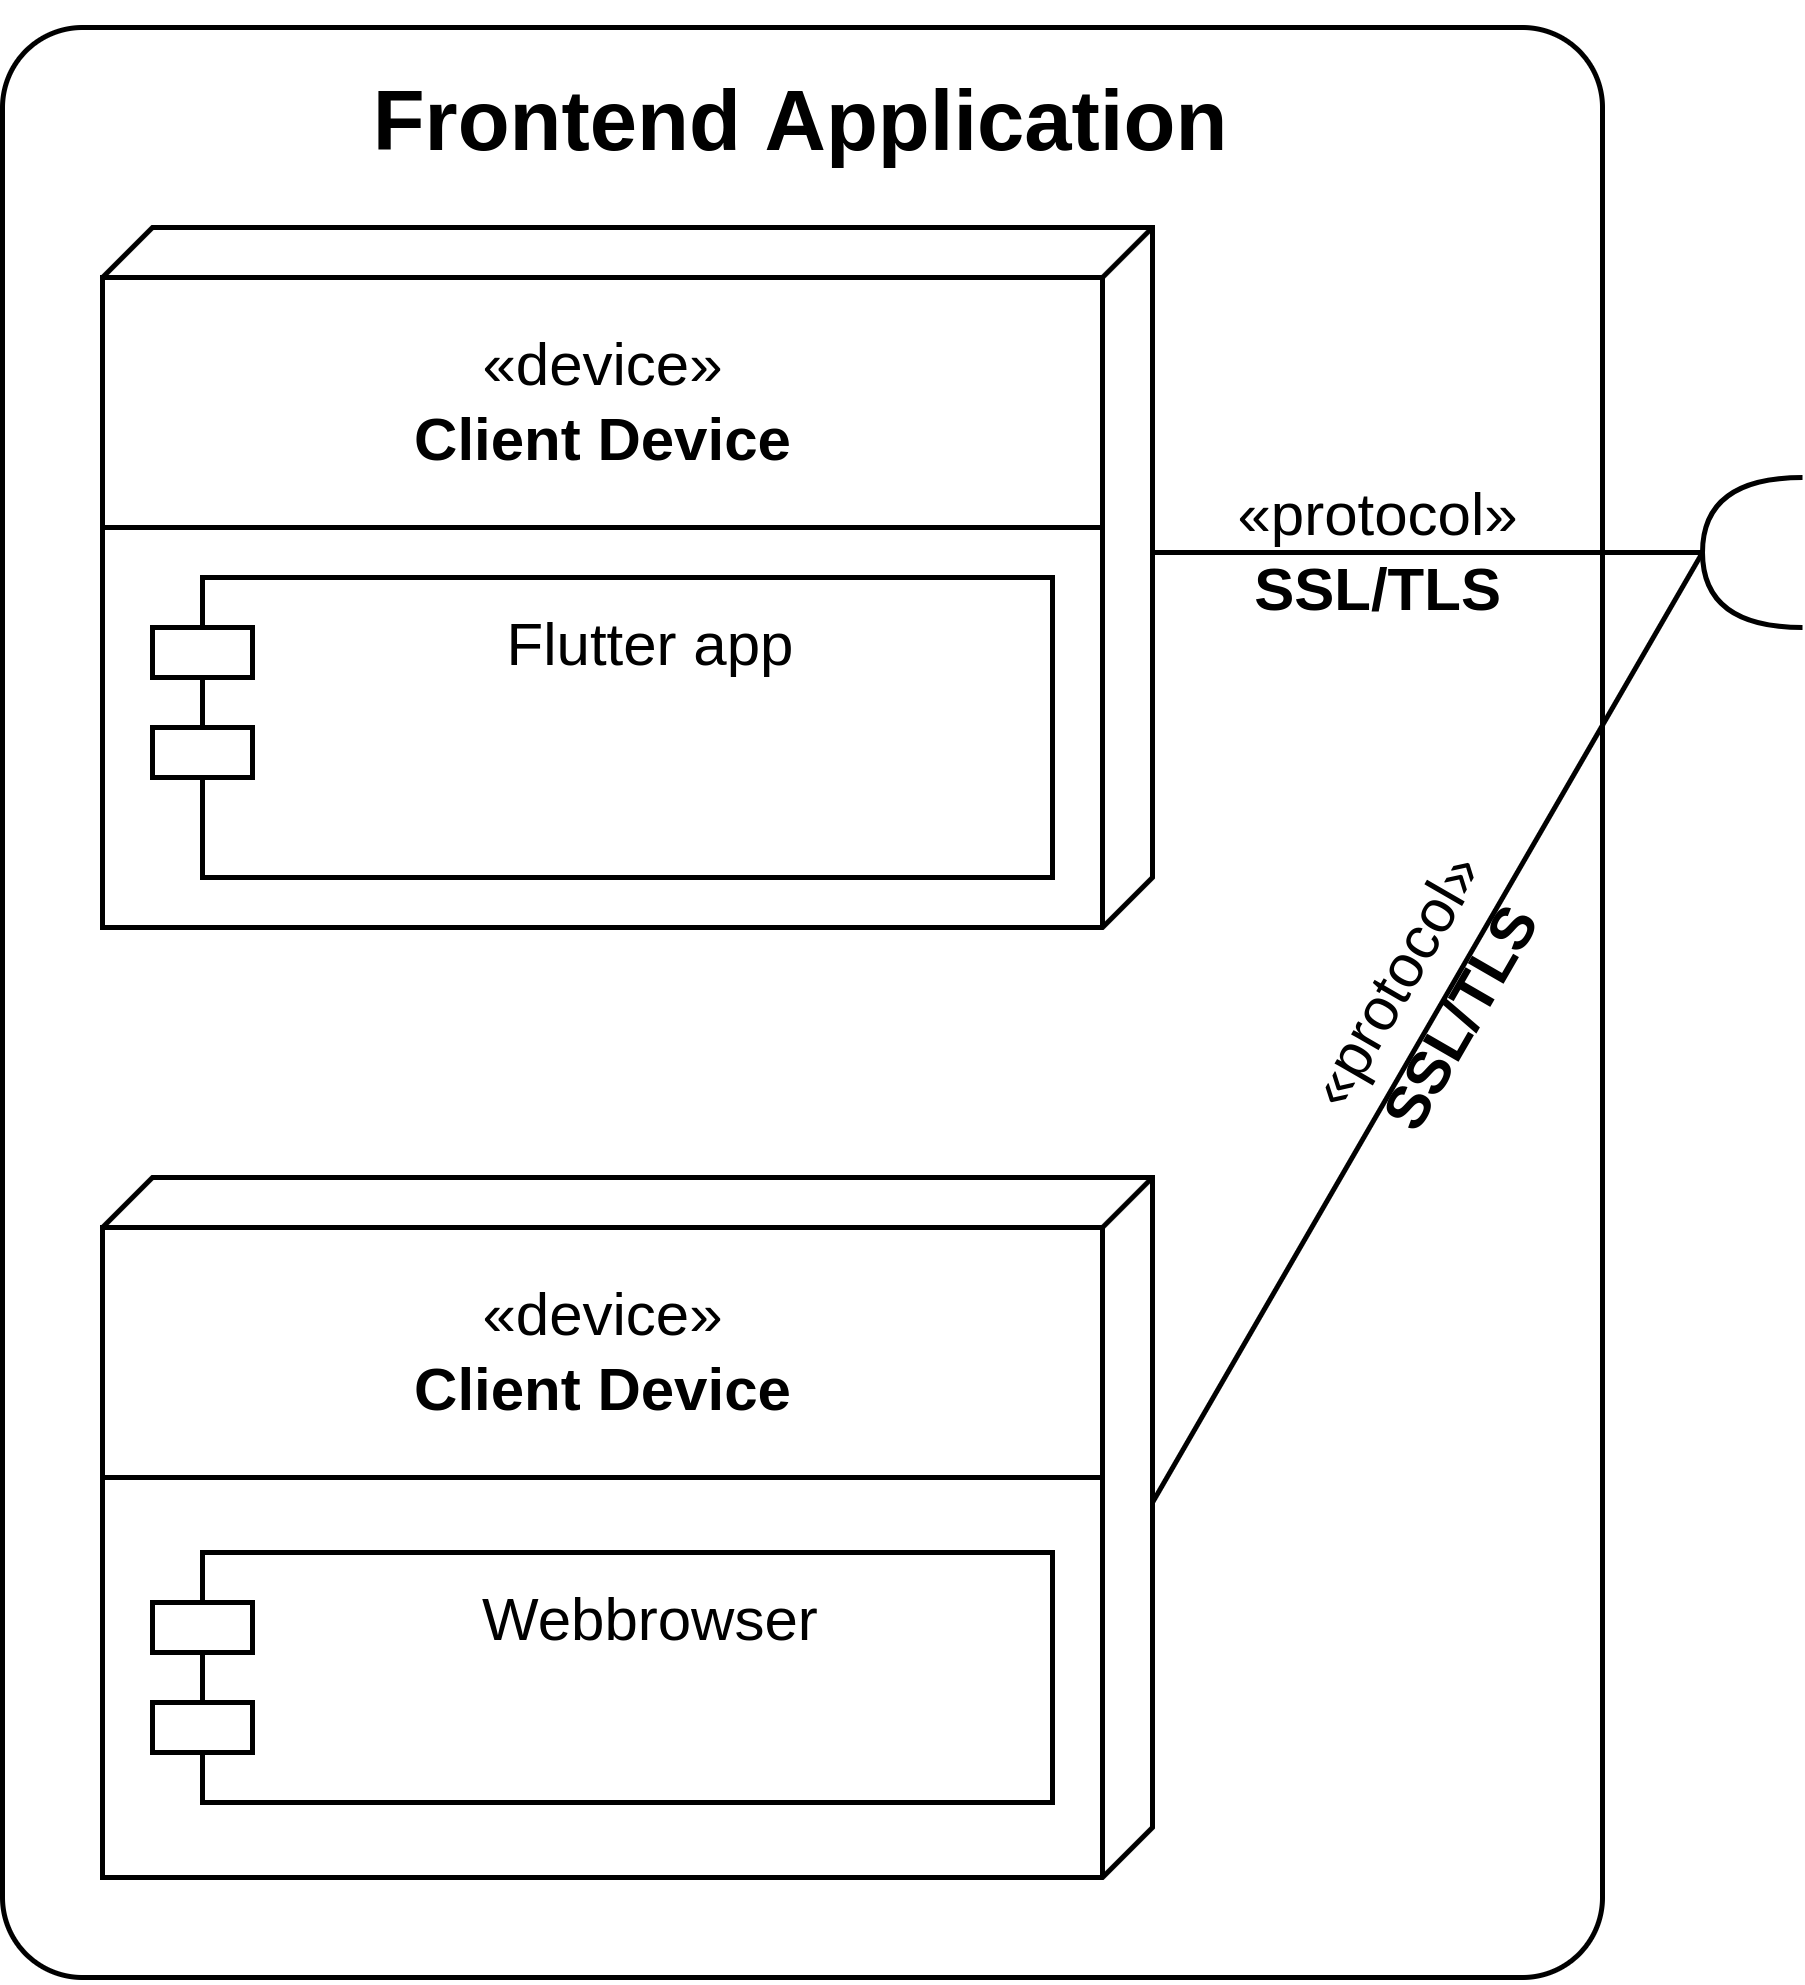
\includegraphics[width=8cm]{images/deployment_diagram_frontend.drawio.png}
    \caption{Deployment diagram of the frontend application.}
    \label{fig:deployment-frontend}
\end{figure}

\subsubsection{Connection to the backend}
The frontend requires some communication to the backend in order to show the user the right information out of the database. This is achieved by using a \ac{rest} \ac{api}, which exposes different URLs to the client. When the client sends a request to one of these URLs an action happens in the backend based on the request. There are four different types of requests implemented in the backend: a get request, a post request, a put request and a delete request. These requests respectively receive, post, change and delete information.

To further explain this communication, the creation of a reservation is a good example. As soon as a user selects a garage, an overview of this garage is given. In order to show this page, a get request is first sent to the \ac{url} of the garage, specified using the index of the garage. This request receives all the information of the garage needed to construct the page shown. Later on when the user has selected a time and date, in order to select a spot another request is sent to the backend. This time also a get request, sent to the \ac{url} concerning the parking lots of a certain garage. A list of parking lots is returned, with their respective state and information. Based on this list, the frontend can build the page for spot selection. After the overview of the reservation, when the user confirms, a post request is sent. This request arrives at the \ac{url} concerning the reservations of the user and a reservation is added to the database. These are just three examples of the many requests sent to the backend in the usage of the frontend and since the latter is not functional without these requests, the communication between front- and backend is very important for the system.


\subsection{Backend}\label{sec:implementation-backend}
The main functionalities of the backend are described in Section \ref{sec:core-functionalities}. This section describes the implementation of those core functionalities. Section \ref{sec:design-motivation} outlines the augments for the different software used in the backend.

\ind The main parts of the backend described below can run on a single physical machine. The deployment of those services can happen both on a local server or on a cloud server. For the purpose of this project, a local home server is preferred, but a real-world system requires scalability which makes a cloud server indispensable.

\subsubsection{Server}
The server is the main entry point to the outside world of the database and the \ac{rest} \ac{api} and thus needs proper security measures. The encryption of traffic happens on the server, origin validation to prevent \ac{csrf}-attacks is included in the backend application (see Section \ref{sec:backend-application}). 

\ind Nginx is used as the main \ac{http}-server in the backend. It serves as an industry standard for a fast and lightweight server. The most important feature for the backend is that it can handle \ac{ssl}/\ac{tls} and redirect \ac{http}-requests to \ac{https}-requests \cite{nginx}. Furthermore, the server has to redirect incoming requests to the right application, namely, the web variant of the frontend application or the backend application. This is achieved via a \textit{proxy-pass}, which can redirect traffic from one server to another, based on certain conditions in the request (e.g. all \acp{url} which starts with \texttt{api/} are redirected to the Gunicorn Python server (see below).

\ind Besides a web server, the backend application needs a way to communicate between the web server and the actual application (in casu the Django application). This is achieved with a \ac{wsgi}. The backend uses Gunicorn\footnote{\url{https://gunicorn.org/}} as its \ac{wsgi}. The main purpose of the \ac{wsgi} is making the deployment more stable and faster. The former is achieved by running multiple instances of the Django application, which improves to overall availability of the system \cite{gunicorn}. Besides improving the deploy stability, the \ac{wsgi} makes it possible to user an Nginx server as reverse proxy for redirecting \ac{http} to \ac{https}-traffic. This is not possible without a \ac{wsgi}.

\ind The services above require a lot of dependencies and configuration files, which can make it tedious to set up on a remote machine. The backend is therefore deployed with Docker containers, which bundles \textit{Docker images} with an \ac{os} in a so-called isolated \textit{container}. This way, all the dependencies are packed inside the container, which eliminates the need of doing a laborious setup on the server machine. In total, there are three containers, one for the Nginx server, one for the Gunicorn gateway which runs the Django application and one for the MySQL database. The containers run as a single service with Docker Compose, which makes communication between the different containers effortless \cite{docker-compose}. Figure \ref{fig:deployment-backend} shows the deployment diagram of the entire backend.

\begin{figure}[htp]
    \centering
    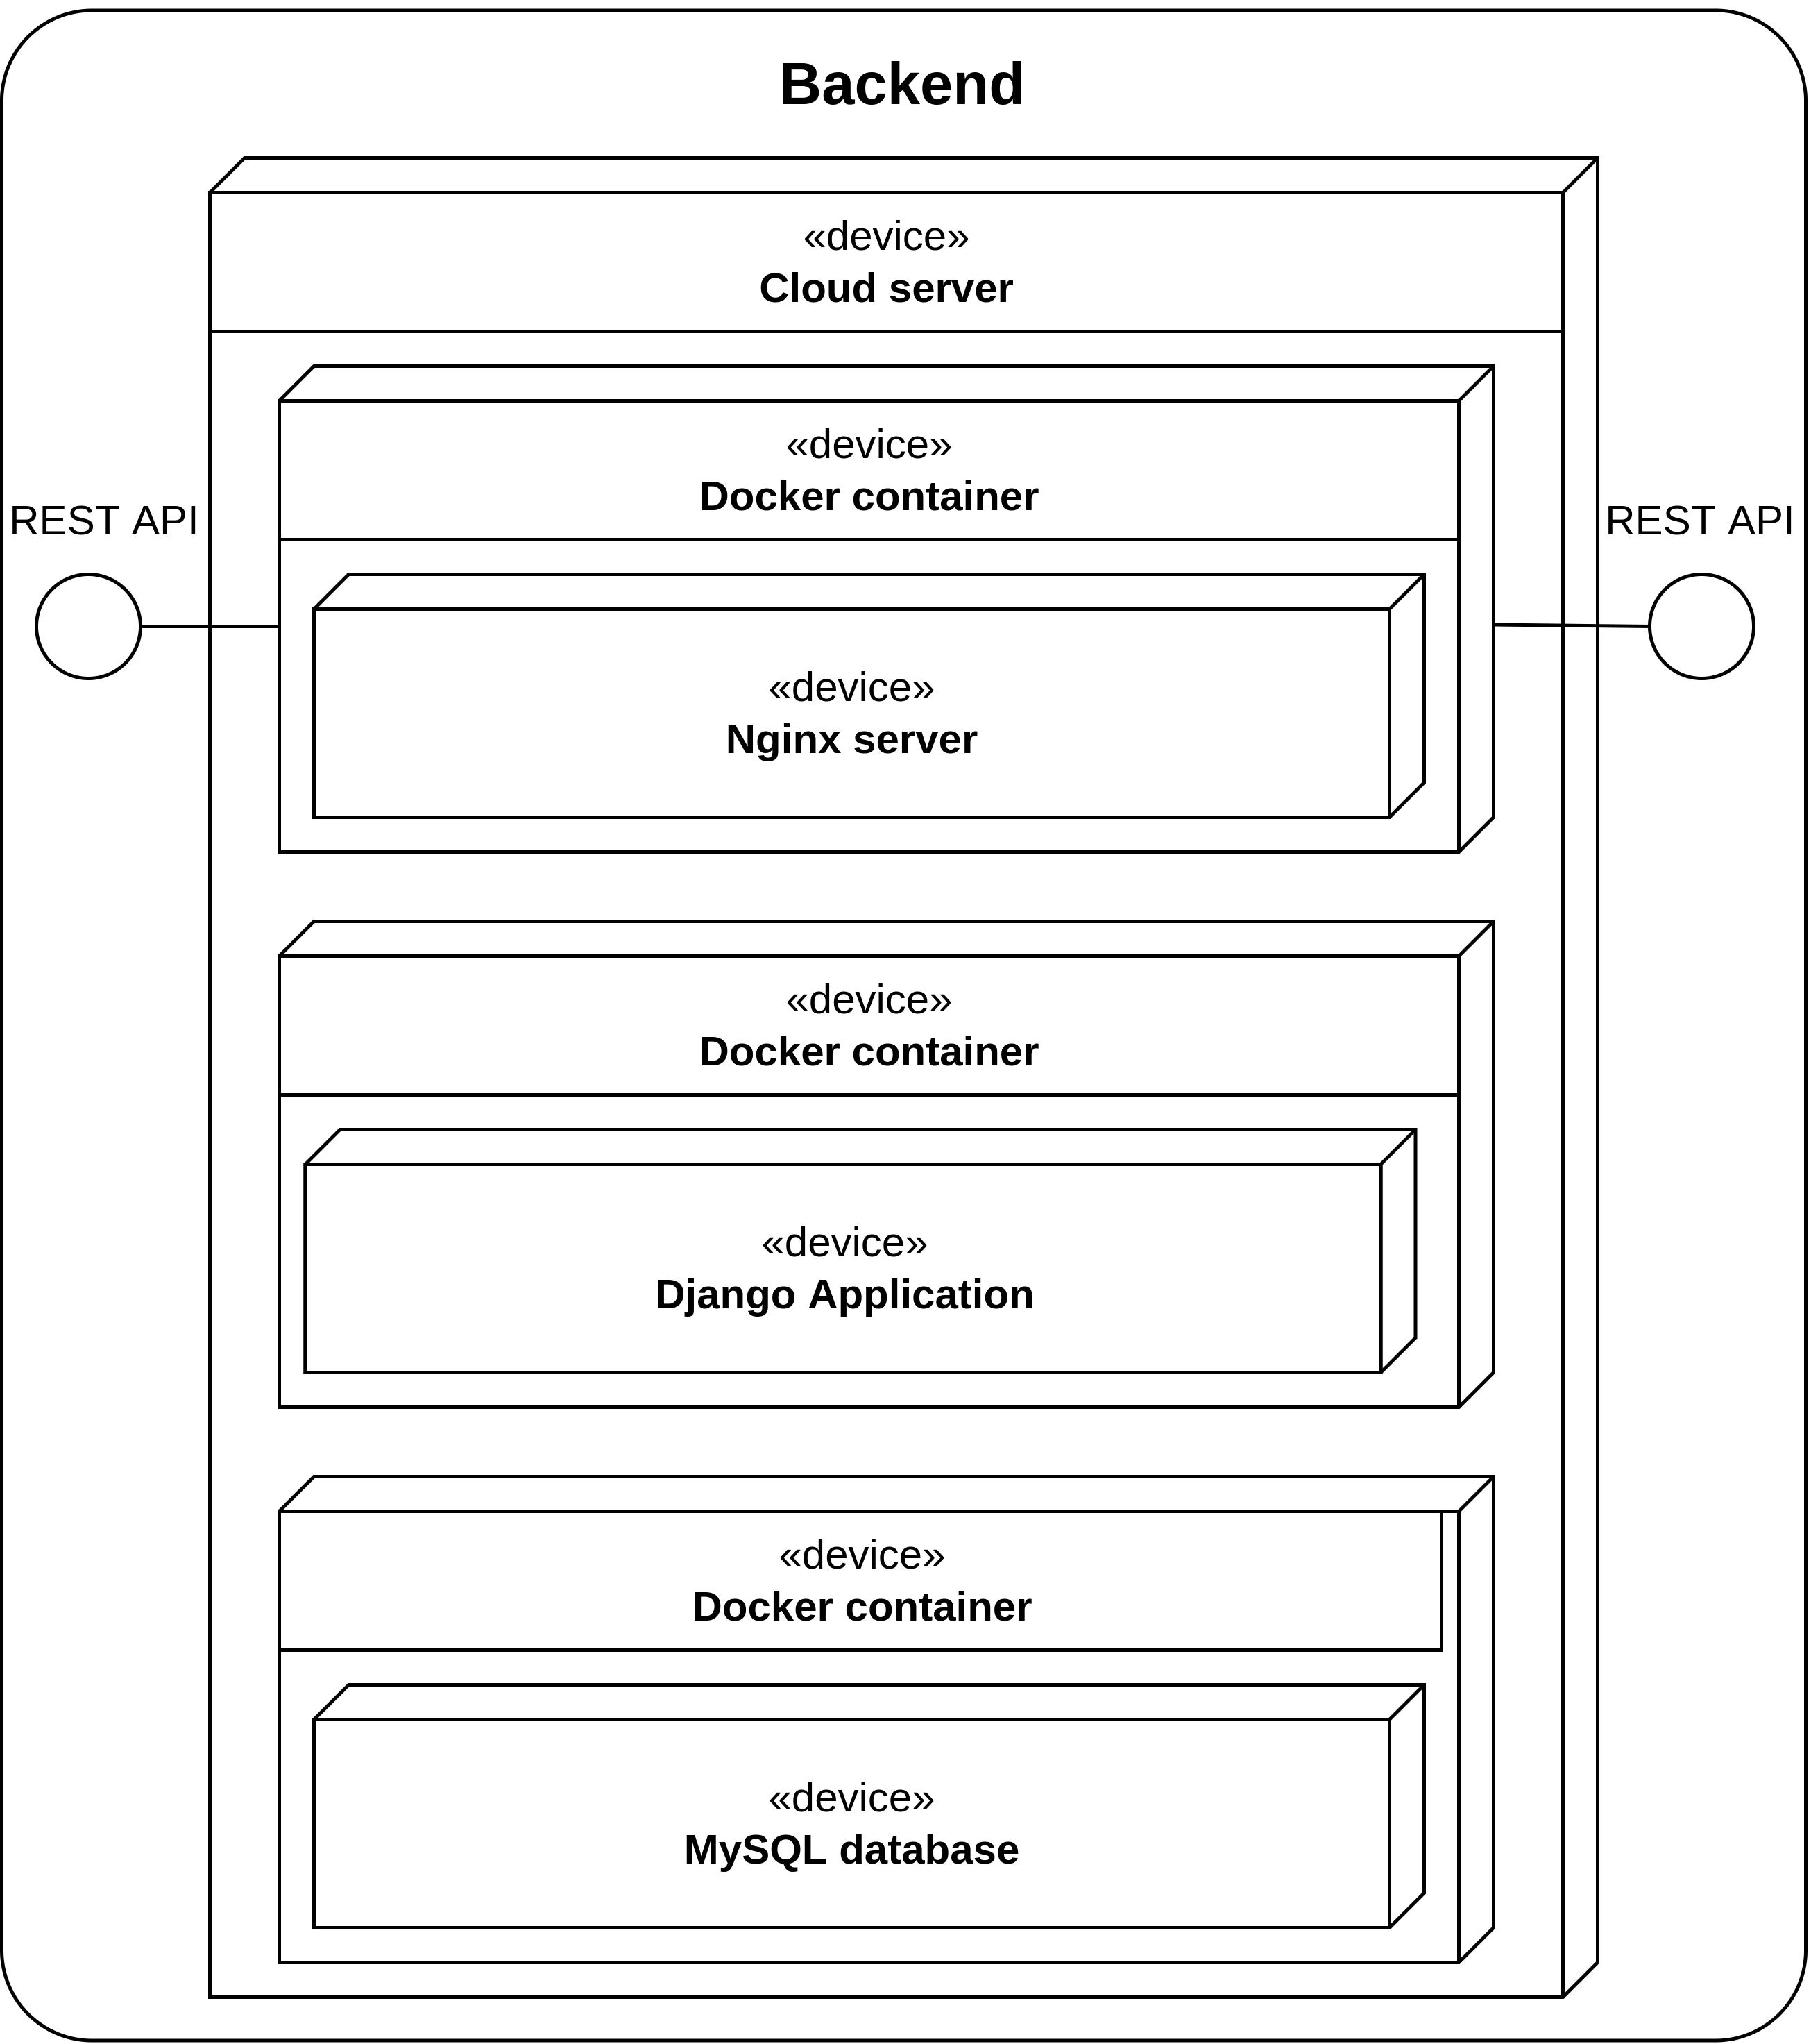
\includegraphics[width=8cm]{images/deployment_diagram_backend.drawio.png}
    \caption{Deployment diagram of the backend server software.}
    \label{fig:deployment-backend}
\end{figure}


\subsubsection{Backend application}\label{sec:backend-application}
The backend server-side application is written in the Django framework. The Django framework serves as an \ac{orm} for the database, which makes it much easier to query the database. The main purposes of the backend application is the retrieve the right information from the database and more importantly, validate if the user is authenticated and authorised to query that information. The database itself is a MySQL, relational database.\footnote{\url{https://www.mysql.com/}} 


\paragraph{User authentication}\label{sec:user-authentication}
User authentication is an essential part of the \ac{ips} in general, due to the fact that this is the primary defence against unauthorised querying of the \ac{api}. The authentication system in the backend consists out of three \textit{views}: registering a new user, logging in a user and logging out an existing user. 

\ind In general, there are three levels of authentication for a user in the backend: \textit{unauthenticated}, \textit{authenticated} and \textit{authenticated and verified}. When a user is not logged is, it is called unauthenticated. If the user has \ac{2fa} enabled and has logged in (meaning a authentication token exists in the database, see further), but has not yet entered their \ac{2fa}-code, it is authenticated, but not yet verified and thus not able to perform any requests. Only if the user has both an authentication and has verified its \ac{2fa}-code it is able to perform requests.

\ind If the user creates a new account with the frontend application, their record will be added to the \texttt{users}-table, but this account is not yet functional. Upon registration an email is sent to the user with an activation link. Once the user has clicked on this link, their account will be activated and can be used to log in.

\ind A user can log in via the frontend application which sends the entered \texttt{email} and \texttt{password} to the backend via a encrypted \ac{ssl}/\ac{tls}-connection. The backend validates the credentials and if they are correct, an \textit{authentication token} is generated and sent back to the frontend. This token has to be used in \textit{all} \ac{api}-requests which query or past data from and to the database. Furthermore, this token indicates if a user is logged in or not. If a token is present in the \verb|knox_authtoken|-table, a user is considered logged in. To prevent attackers to log in with this token from a separate device, the number of tokens is limited to one token per user. If someone tries to log in with the credentials of an already logged in user, an error is returned. This token also makes it possible for the frontend to implement an automatic login system for the users.

\ind From the frontend application, users are able to log themselves out. From a backend's perspective, this means deleting the authentication token from the database. In order for the logout the succeed, the authentication token has to be sent with the request. This prevents unauthorised logging out of users. 

\paragraph{Serialization of database models}\label{sec:backend-serialization}
All data is transmitted in \ac{json}-format in the \ac{api}, but it cannot be directly inserted in this format in the database. One of the tasks of the backend application is \textit{serializing} the data between the \ac{json}- and database formats. This not only happens when data is queried from the database, but also when data is posted to the \ac{api}. In this direction, the serializing function becomes more important, because it \textit{validates} the sent data. The data has to match the requirements of the schema of the database (e.g. certain columns of the database are non-null, others have to be unique, etc.). If not, an error message is returned to the sender and the record will not be stored. This procedure is also the main defence against \ac{sql}-injection.

\ind On the backend level, models are related to each other, which makes it possible to build complex data structures. Possible relations are \verb|has_many| or \verb|has_one|, which indicates that a parent model can have multiple or only one child model, respectively. Figure \ref{fig:class_diagram} shows a schematic overview of these relations. 

\begin{figure}
    \centering
    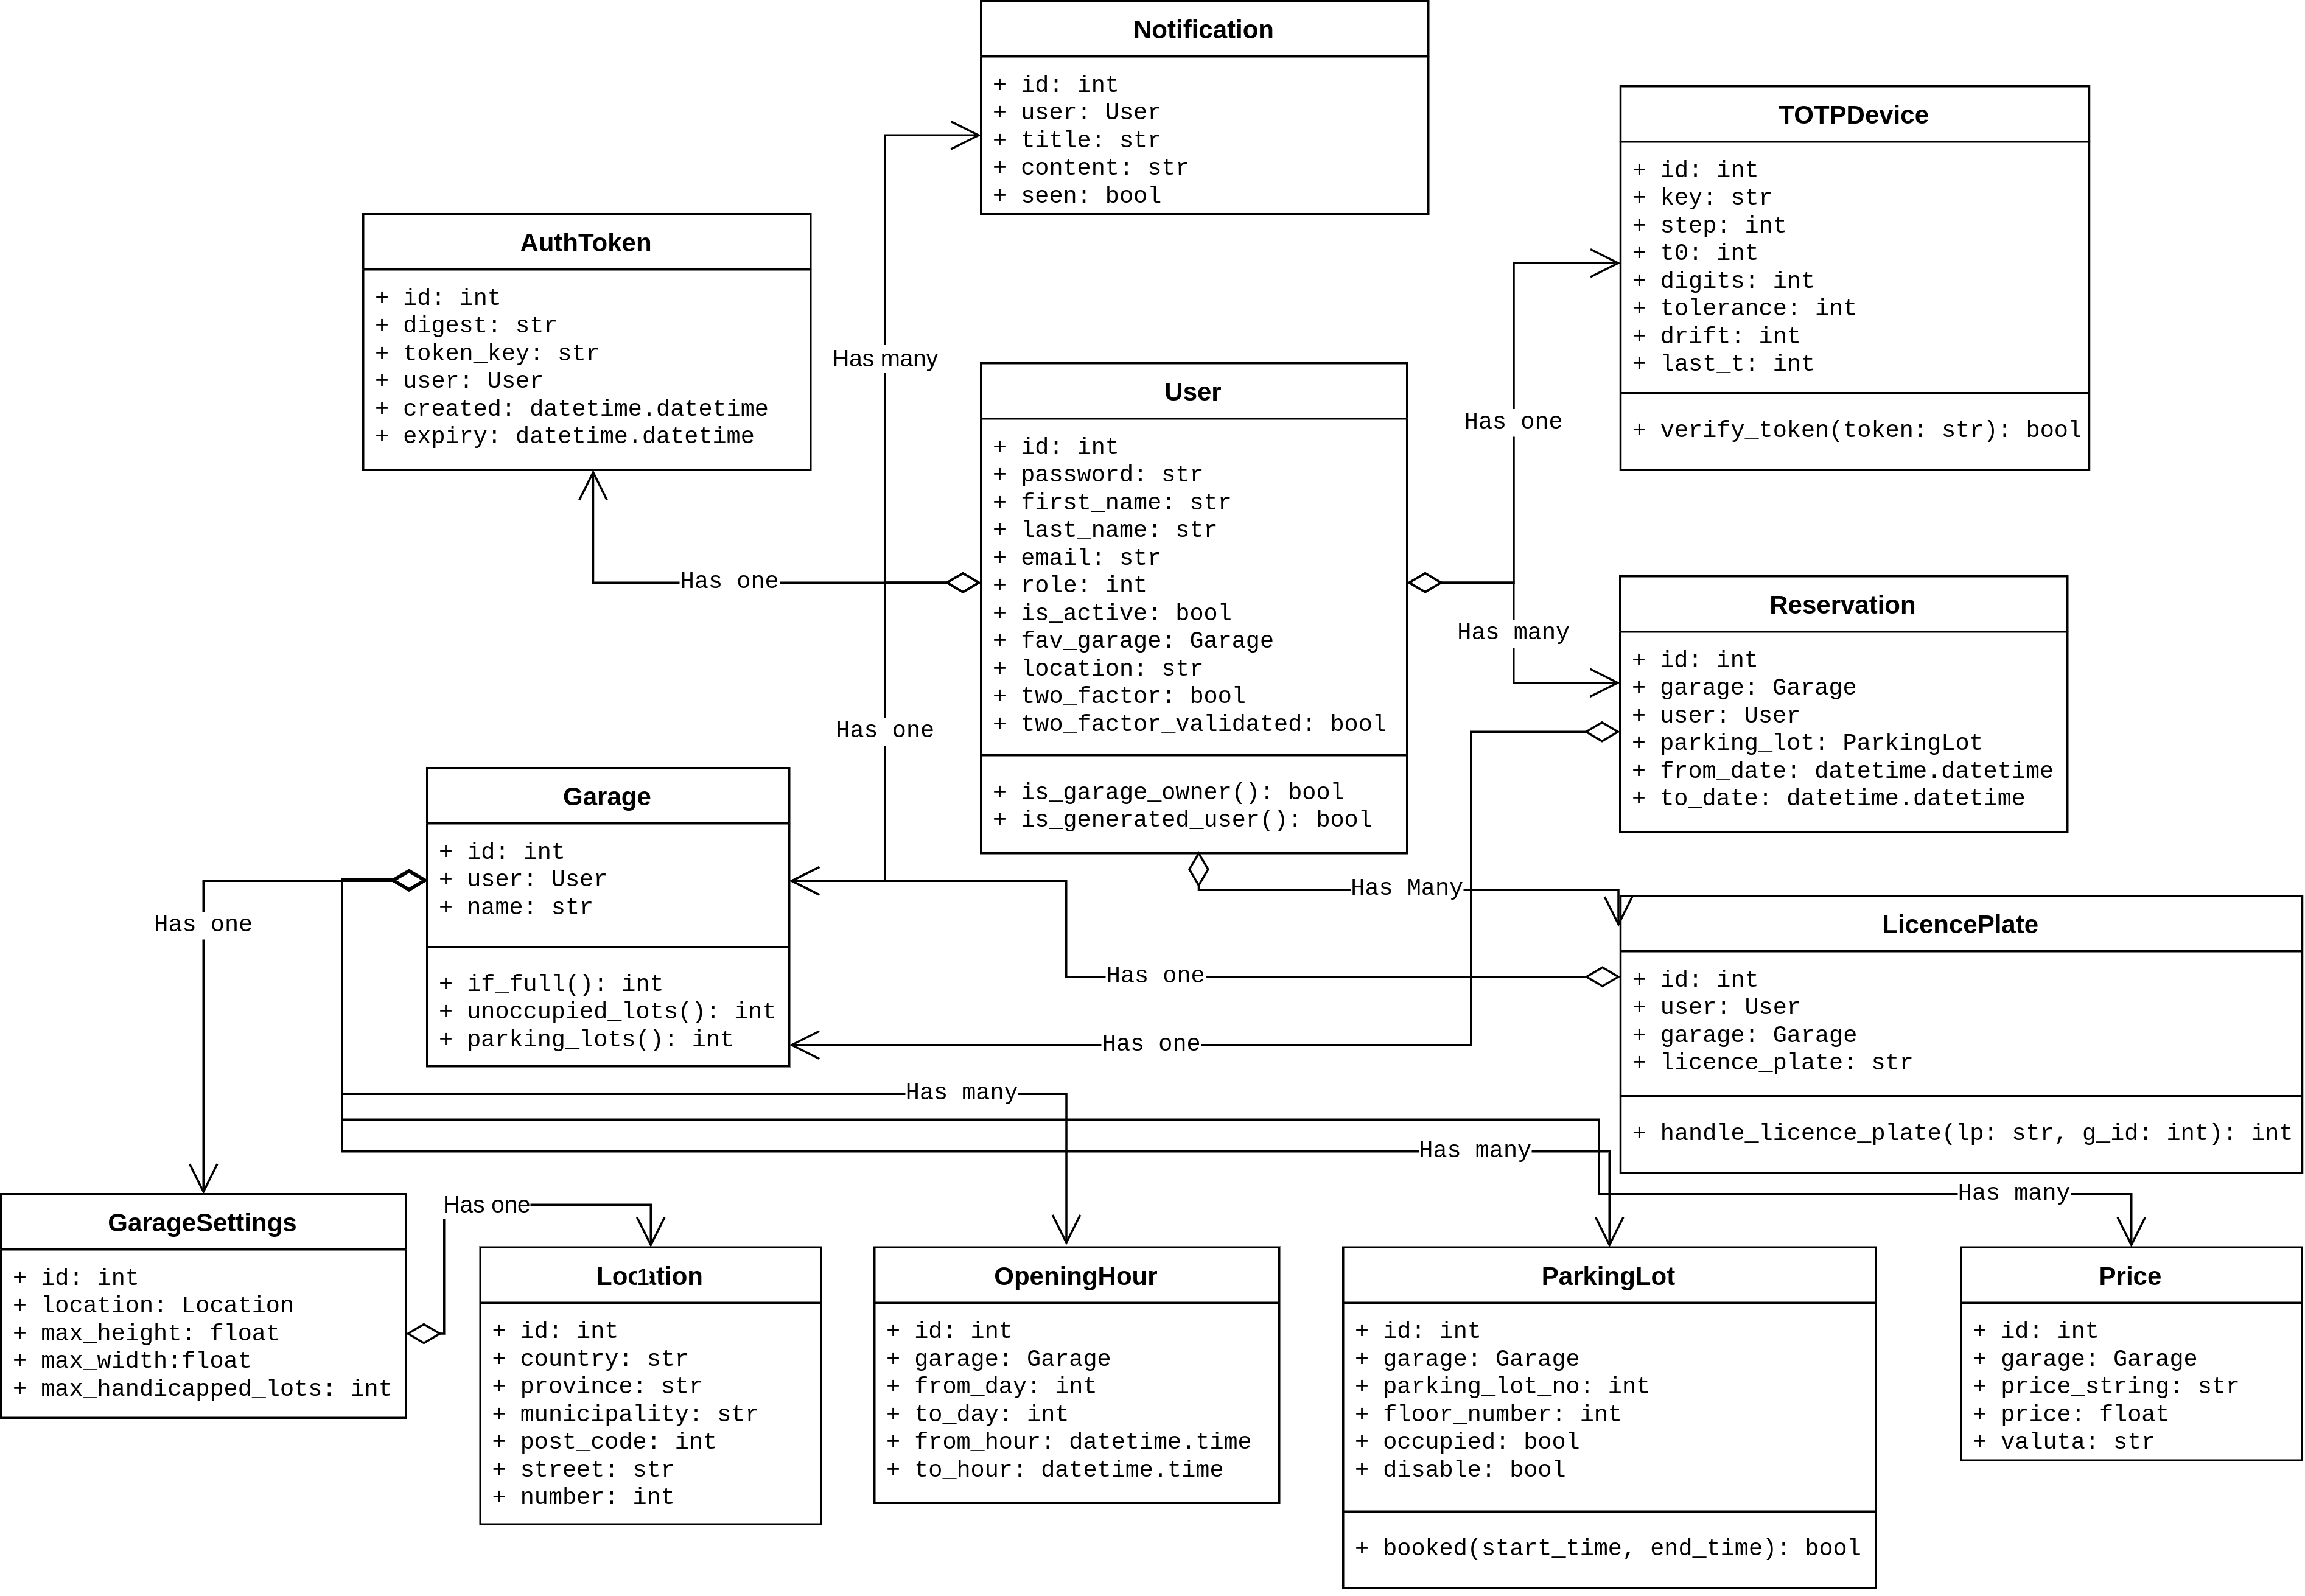
\includegraphics[width=10cm]{images/class_diagram.drawio.png}
    \caption[Class diagram of the backend.]{Class diagram of the backend, which shows the relations between the different models. Note that the relations are only marked one-way, while they exist both ways in practice.}
    \label{fig:class_diagram}
\end{figure}

\paragraph{User roles}\label{sec:backend-roles}
All users in the database have one specific role, which is associated with a set of \textit{permissions} for this user. There are three roles: \verb|GENERATED_USER|, \verb|NORMAL_USER| and \verb|GARAGE_OWNER|. Upon registration with the frontend application, the default role is \verb|NORMAL_USER|. In order for a user to register as a \verb|GARAGE_OWNER|, the user has to provide the necessary legal documents which proves its ownership of a garage. The set of permissions of the \verb|GARAGE_OWNER| is a superset of the user permission set, with the added permissions of adding and deleting garages and adding, disabling and deleting parking lots.

\ind The \verb|GENERATED_USER| is a special role which is created upon entering of a user without an account in the parking garage. The \ac{anpr}-cameras send registered text of the licence plate to the backend. Then the backend checks if the licence plate is already registered in the database. If not, a new dummy user, with the role \verb|GENERATED_USER| is created with the associated licence plate. This account only serves as a visualisation of the parameters of the user's park (e.g. duration) and has no functionalities which are found in a normal user's account. Upon exiting of the garage, the backend checks the associated role of the user; if it is a \verb|GENERATED_USER|, the account, with the associated licence plate, is deleted.

\paragraph{Automatic number plate recognition}\label{sec:anpr}
The backend implements \ac{anpr} to identify cars coming in and out of the garage. It is performed on the image which is sent to the backend via the Raspberry Pi (see Section \ref{sec:entrance-system}) Its goal is to reliably detect the licence plate from different angles, light conditions and quality of the image. There are multiple ways to solve this problem. It is possible to use machine learning, however this requires a large dataset of good quality images to train the model. Creating these datasets takes a lot of resources, so this approach is out of the scope for this project. Another way to detect the text on the licence plates is to firstly find the licence plate on the image and then read the text in the region of the licence plate \cite{anpr}. The advantage is that there are already publicly available \ac{ocr} tools to find text in images. 

\ind The licence plates can be located because of their predictable shape. They are rectangular with a certain range of possible aspect ratios and have mostly contrasting colours. Therefore, an algorithm can find candidates of licence plates by converting the image to greyscale and applying a threshold on it. The image now only has black and white pixels, indicating the dark and light regions. In these pixels it can then look for rectangular regions. Out of these candidates, the algorithm can select the real licence plate based of the (amount of) text on it. It can also filter them based on given licence plate formats. In Belgium, for example, most licence plates have the `1-ABC-123' format. The filters can be changed easily because it is an argument to the OCR-function. This approach will not work in real applications because of unknown formats or custom licence plates but this approach is sufficient for this project.

\ind To read the text on the licence plates, two \ac{ocr} tools are used: EasyOCR \cite{easyocr} and Google Vision \ac{api} \cite{googlevision}. EasyOCR is free but less accurate, this is perfect for filtering out the licence plate candidates without any text on it. Google Vision \ac{api} is a paid service, it costs \$1.5 for 1000 requests with 1000 free requests per month, but it is almost error-free. Google Vision is only used on the final candidate to stay below these 1000 requests.

\paragraph{Payment}
The backend supports two main payment options: manual payments and automatic payments. For the manual payments, users can use all mainstream payment methods (e.g. Bancontact, iDeal), for automatic payments only card payments are supported. All payments are handled by the Stripe platform.\footnote{\url{https://stripe.com}} They provide simple integration of more payment methods, as well as an easy to use dashboard to get an overview of all payments. This project uses their checkout (manual payments) and invoice (automatic payments) \acp{api}. 

\ind When a user wants to pay, the backend has to know how much it should charge, regardless of the payment method. It calculates the required amount based on the prices of the garage stored in the database and the duration for which a user is parked. The garage can have multiple prices, each based on a different parking duration. To get the best price the algorithm starts with the price with the longest duration and subtracts it from the parking time as much as possible, then the same thing happens for the next price and so on. For example, when there are prices for 1 day, 8 hours and 1 hour present in the database, and the user parked for 12 hours, they have to pay the price for 8 hours once and the price for 1 hour four times. The cumulative amount is then charged to the user.

\ind The manual checkout can be used by all users. When a request for manual payment is sent to the backend, it sends all the prices and their quantities (as explained above) to Stripe. Stripe subsequently creates a checkout \ac{url}, which is then returned by our backend as well. Finally, the frontend redirects the user the checkout page using the requested \ac{url}.

\ind To use automatic payments, a user has to add a card to their account. This can be done by sending the necessary details (card number, expiration date and \ac{cvc} code) to the backend.\footnote{Note that the backend \textit{does not} store these credentials. They are only needed to create a customer at Stripe, where after they are deleted from the backend systems.} After that, a new customer is created on Stripe, this is necessary for storing the new card payment method. When a user with a connected card tries to leave the garage, the backend can automatically charge the card using the invoice \ac{api} and the customer on Stripe. 

\ind The backend can detect succeeded or failed payment attempts using \textit{webhooks}.\footnote{Webhooks are functions which can be called based on certain events happening on the web page, e.g. a user making a payment.} This means that \textit{Stripe} will make a request to the backend \ac{api} for each new event. When the payment was successful, the licence plate of the user is updated so that it can leave the garage. If the payment failed, the backend sends an email to the user with a new payment \ac{url}.


\subsubsection{Security}\label{subsec:sucurity}
As explained in Section \ref{sec:core-functionalities} security is on the most important aspects of the backend. Of course, security is not limited to the backend alone, as it is often a conjunction between the frontend and the backend

There are numerous attacks possible against a backend service, so it is not possible to list them all. The following sections will describe the most common vulnerabilities and how they are prevented. Table \ref{tab:backend-security} gives a schematic overview of the following paragraphs.

\paragraph{Injections attacks}
Generally, during an injection attack, an attacker will try to inject malicious input in the backend system, most often done via the frontend application, which allows user to input data \cite{injection_attacks}. The most common types are \ac{xss}, in which the attacker tries to input (most-often \ac{js}) code into the remote server and \ac{sql} injection, in which the attacker tries to input \ac{sql}-commands into the server.\footnote{Note that there are many more possible injection attacks, like buffer overflows, format string attacks and command injection, etc.} If any of these succeed, it can lead to the \ac{rce}, which makes the sever vulnerable for leaking sensitive information or to redirect users to the malicious sites. Depending on the severity, an attacker is able to perform any command on the server. The primary defence  against injection attacks is sanitising of user input.\footnote{Note the difference between \textit{serializing} (see Section \ref{sec:backend-serialization}) and \textit{sanitising} data.  The former is needed for compatibility between the frontend and the backend, the latter is an essential tool for preventing injection attacks.} This includes escaping any non-alphabetic characters. A second key point is setting a max-length on \textit{all} input fields, in which the user can enter data. This specifically prevents database corruption through memory corruption.

\paragraph{\acp{acm}}
From a backend's perspective, there are three \acp{acl}, associated with the roles, described in Section \ref{sec:backend-roles}. Each \ac{acl} has a strict associated set of permissions, which prevents that users perform actions which they should not perform (e.g. altering information about a garage) and that users cannot alter object, on which they have no ownership (e.g. altering information about a different user). The backend is designed in such a way that requests that the user parameter is determined automatically from the authentication token, without sending it directly with the request. This prevents \ac{idor} and the malicious editing of objects. 

\ind Apart from determining the user automatically from the request, the backend implements an additional set of permissions to the role \verb+GARAGE_OWNER+. They are allowed to add garages and parking lots to the system, as well as to alter or delete garage and parking lots which they own.


\paragraph{Request Forgeries}
\ac{csrf}-attacks and \ac{ssrf}-attacks are different, but related attacks which are caused by a lack of origin validation with the server. In the former, an attacker misuses the user credentials to performs actions as if the attacker was the user, in the latter the attacker targets services which are running internally on the server, causing it to leak sensitive information.

\ind The backend implements a rigorous origin-validation system, with the use of \ac{jwt}-tokens.\footnote{\url{https://jwt.io}} Each time a request is made, the frontend application will generate a new \ac{jwt}-token and signed with a secret key only known to the backend server and the frontend application. The \ac{jwt}-token only lives for 5 seconds, preventing the capture and re-use of tokens. 

\ind Based on the deployment diagram, the backend has to be able to accept requests from two different origins: the local garage system and the frontend application. All requests from any other location are rejected. This prevents both types of attacks mentioned above: if the attacker gets hold of the user's authentication token, he/she will not be able to perform any requests with it, as only the frontend application can send valid request to the backend server. Furthermore an attacker will not be able to gain access to internal services running on the server as it is only accessible via the frontend application, which can only interact with the Django framework.

\ind The origin-validation of local garage system proceeds in a similar fashion, but the \ac{jwt}-token has no expiry, as it cannot be intercepted as the data is send via \ac{https} and thus the sent data as well as the cookies are encrypted. This further prevents \ac{mitm}-attacks.

\paragraph{Other security measures}
Apart from the above measures taken to enhance security of the backend, the backend also obliges users to choose strong passwords\footnote{The backend demands that a password is at least 10 characters long, contains a capital letter, a numerical symbol and a special character and may not be associated with any user information.} and allows the use of \ac{2fa}. Once the user is logged in, he/she can add a \ac{totp}-device. The backend then returns a security code which the user can enter in \ac{tpa} like Google Authenticator. From then on the user has to be both \textit{authenticated} and \textit{verified} to perform any requests. 

\ind The backend also requires the users the validate their email address given at sign up. If the user signs up, their object will be added to the database, but it will be inactive. Users will not be able to log in until they activate their account. This limits the creation of accounts with false email addresses.


\begin{table}[htp]
    \centering
    \begin{tabular}{|c|c|}
         \hline
         \textbf{Attack}& \textbf{How prevented?}  \\
         \hline
         \hline
         \ac{sql} injection & Serializing all user input. \\
         \hline
         \ac{xss} & Serializing all user input (also in the frontend application).\\
         \hline
         \ac{idor} & User data requests return only info about the current user. \\
         \hline
         \ac{acm} & Strict \ac{acl} with added permissions. \\
         \hline
         \ac{csrf} & Use of a strict origin validation policy with \ac{jwt}-tokens. \\
         \hline
         \ac{ssrf} & Use of a strict origin validation policy with \ac{jwt}-tokens. \\
         \hline
         \ac{mitm} & Use of \ac{https}. \\
         \hline
         Brute force & Rigorous password policy \\
         \hline
         Stolen password & Possibility of \ac{2fa}. \\ 
         \hline
    \end{tabular}
    \caption{Overview of the backend's security measures against different attacks.}
    \label{tab:backend-security}
\end{table}


\subsubsection{Privacy}
Besides security, privacy is another core functionality of the \ac{ips}. As the backend is responsible for storing sensitive information about the user, it is most suited to build a solid privacy policy.

\paragraph{Least to know principle}
The backend implements the so-called `least to know principle`, which indicates that it only stores the information it actually needs to function properly. All other data is or not stored in the backend data (e.g. credit card details of the user) or deleted from the moment the data becomes irrelevant (e.g. information about a user's reservation is deleted two hours after the reservation is finished). Even in the event of a data breach, no relevant information about a user can be obtained. Other sensitive information, like passwords are hashed before they are stored in the database.

\paragraph{Licence plate validation}\label{sec:licence-plate-validation}
Some current parking application make it possible for people to be followed based upon their licence plate \cite{privacy_breach}. This is a major privacy breach. In the frontend application, users can add a licence plate to their account, but it is not activated (and cannot be used to make reservations) until they submit a valid vehicle registration document proving the ownership of their licence plate. Furthermore, the \verb|licence_plate|-column has to be unique, meaning that it is impossible for different users to add the same licence plate to their account. The frontend application provides an additional possibility to report a licence plate if a user thinks that someone else has registered their licence plate.

\paragraph{Anonymous use}
The backend also fully supports anonymous use of the \ac{ips}, without giving in to user-friendliness. 
It is possible that a user drives towards a garage, without having the account and without having the application installed and yet have a similar parking experience as users with an account and in complete anonymity. In the before described case, the backend will generate a user with the associated detected licence plate. The local garage system will print out a paper ticket with an \ac{qr}-code on it. Scanning this \ac{qr}-code opens the frontend application, hosted on the Nginx-server, with the user already logged in with the generated account.  This account allows the user to see in which garage they are parked, the time they are parked and a way to pay the due amount. Upon exiting of the garage, this account, with the associated licence plate will be fully deleted from the database. From a backend's perspective, the park ceases to exist to moment the user exits the garage, which renders it untraceable.